La necesidad de contar objetos y animales genera la necesidad de asociarlos con números, los primeros conocidos son los Números Naturales cuya notación es $\mathbb{N}$:
\[ \mathbb{N}=\{ 1,2,\dots\} \]
Una de las propiedades de los naturales es que cada número tiene un siguiente $\operatorname{sig}(n)$, así el siguiente a $1$ es $2$, el siguiente de $5$ es $6$, y así sucesivamente, en general dado el número natural $n$ el siguiente será $n+1$.

Además de permitirnos contar, con estos números se pueden resolver algunas ecuaciones asociadas a una primera operación elemental, la adición, por ejemplo hallar el valor de $x$ que cumpla:
\[ x+3=5 \]
cuya solución es \fbox{$x=2$} pues al reemplazar la variable $x$ por $2$ en la ecuación, resulta: $\fbox{2}+3=5$. De la misma forma, la ecuación $5x=15$ tiene como solución $x=3$.

Sin embargo, al tratar de resolver esta otra ecuación:
\[ x+4=1 \]
Encontramos que NO tiene solución en los naturales, es decir que ningún natural satisface la ecuación puesto que la solución corresponde a $x=-3$, el inverso aditivo del número natural $3$, no obstante no hace parte de los naturales $(-3\notin\mathbb{N})$. Es necesario considerar un nuevo conjunto que incluya los naturales, sus inversos aditivos y el cero. Tal es el conjunto de los números enteros denotado por $\mathbb{Z}$:
\[ \mathbb{Z}=\{\dots -2,-1,0, 1,2,\dots\} \]

\section{Operaciones elementales}
A continuación se presentan las operaciones en los naturales y algunas de sus propiedades:

\subsection*{Suma}
La operación suma en los naturales no reviste mayor complejidad, en los enteros $\mathbb{Z}$, vamos a tener una convención, para sumar dos enteros del mismo signo se suman y se deja el signo de los dos, así por ejemplo $-2-3=-5$, ahora, si los enteros son de signos distintos, se realiza la resta normalmente y se coloca el signo del mayor, veamos, $-4+1$, se hace la resta $4-1=3$ y se coloca el signo del mayor así que el resultado es $-4+1=\fbox{-3}$, presentado en una recta lo que estamos haciendo se puede ver en la figura (\ref{fig:restaenteros}), partiendo de $0$, nos vamos $4$ unidades hacia la izquierda esto es $-4$ y luego una unidad hacia la derecha $+1$ después de los dos movimientos quedamos ubicados en $\fbox{-3}$ que es el resultado final:

\begin{figure}[ht]
\begin{center}
\caption{Resta de Enteros}\label{fig:restaenteros}
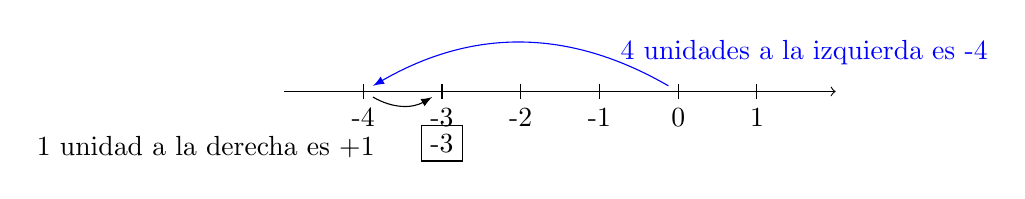
\begin{tikzpicture}[scale=1]
\draw[->] (-5.0,0.0) -- (2.0,0.0);
\foreach \x in {-4,-3,-2,-1,0,1} \draw (\x,0.1)--(\x,-0.1) node[below] {\x};
\node[below] at (-3,-0.3) {\fbox{-3}};
\node (B) at (0,0) {};
\node (M) at (-4,0) {};
\node (P) at (-3,0) {};
\draw[blue,->,>=latex] (B) to[bend right] (M);
\draw[->,>=latex] (M) to[bend right] (P);
\node[blue] at (1.6,0.5) {4 unidades a la izquierda es -4};
\node at (-6.0,-0.7) {1 unidad a la derecha es +1};
\end{tikzpicture}
\end{center}  
\end{figure}

\begin{ejemplo}[Adicional: Suma en la recta]
    Si tenemos $2 + (-5)$, partimos de 0, avanzamos 2 a la derecha y luego retrocedemos 5 a la izquierda. Llegamos a $-3$.
    \[ 2 + (-5) = -3 \]
\end{ejemplo}

\subsection*{Producto y División}
A continuación se presentan aspectos relevantes del producto y la división de naturales y enteros:

\begin{enumerate}
    \item \textbf{Múltiplo:} Dado un número natural $k$, se dice que $m$ es un múltiplo de $k$ si existe $n\in \mathbb{N}$ tal que $m=kn$, así por ejemplo $6$ es múltiplo de $2$ porqué existe el número $3\in \mathbb{N}$ tal que $6=2\times 3$. Si se multiplica un natural $k$ por todos y cada uno de los números naturales resulta un conjunto denominado ``múltiplos de $k$'' que lo notaremos $M(k)$, así por ejemplo si queremos hallar los múltiplos de $2$, éste se multiplica por cada uno de los naturales, se obtiene:
    \[ M(2)=\{ 2,\ 4,\ 6, \dots \} \]

    \item \textbf{Algoritmo de Euclides (Algoritmo de la división):} Si por ejemplo se quieren repartir $11$ objetos entre $4$ personas, el proceso se hace por medio de restas sucesivas. Los $11$ elementos son el ``dividendo'' $D$, serán repartidos equitativamente entre $4$ personas o grupos, lo llamaremos el ``divisor'' $d$, a la cantidad de objetos que se entreguen a cada persona lo denominamos el ``cociente'' $c$, y al número de elementos sobrantes, o aquellos con los que no se pueden completar grupos completos, se llamará el ``residuo'' $r$.
    
    En la figura (\ref{fig:divisionlarga}) se muestra un resumen del proceso:
    \begin{figure}[ht]
    \centering
    \opidiv[displayintermediary=all, voperation=top]{11}{4}
    \caption{División Larga.}\label{fig:divisionlarga}
    \end{figure}

    Vemos una representación gráfica de la división en la figura (\ref{fig:divisiongraph}), así para hacer $11\div 4$, a cada persona (círculos de la figura) le corresponden $2$ objetos osea el cociente, al tratar de repartir los tres objetos restantes vemos que no es posible darle a cada persona otro objeto adicional, ``pues alguien se quedaría con uno menos!!'', por ésta razón el resultado será que a cada persona le corresponden dos objetos y del total sobran $3$ elementos que corresponde con el residuo.
    
    \begin{figure}[ht]
    \begin{center}
    \caption{División por restas sucesivas.}\label{fig:divisiongraph}
    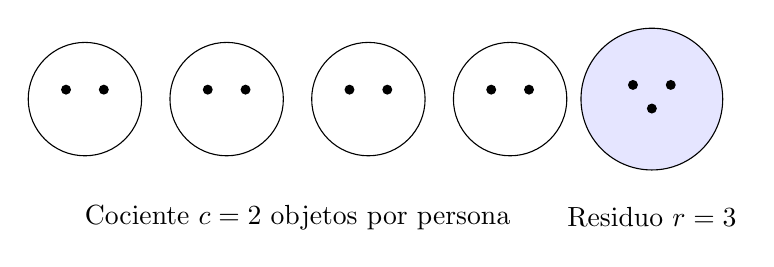
\begin{tikzpicture}[scale=0.6]
    \foreach \x in {-4,-1,2,5} {
        \draw (\x,0) circle [radius=1.2cm];
        \fill (\x-0.4,0.2) circle (3pt);
        \fill (\x+0.4,0.2) circle (3pt);
    }
    \node at (0.5, -2.5) {Cociente $c=2$ objetos por persona};
    \draw[fill=blue!10] (8,0) circle [radius=1.5cm];
    \node at (8, -2.5) {Residuo $r=3$};
    \fill (7.6,0.3) circle (3pt); \fill (8.0,-0.2) circle (3pt); \fill (8.4,0.3) circle (3pt);
    \end{tikzpicture}
    \end{center}  
    \end{figure}

    La división también la podemos representar como en (\ref{eq:divisionum}) así\footnote{En algunas ocasiones $2+\frac{3}{4}$ se escribe $2\frac{3}{4}$ y se lee ``dos enteros tres cuartos''.}:
    \begin{equation}\label{eq:divisionum}
         \frac{11}{4}=2+\frac{3}{4}
    \end{equation}

    En términos generales el algoritmo de Euclides se puede escribir como en (\ref{eq:euclides1}) y se leerá, dividendo ``D'' sobre divisor ``d'' es igual al cociente ``c'' más el residuo ``r'' sobre el divisor.
    \begin{equation}\label{eq:euclides1}
         \frac{D}{d}=c+\frac{r}{d}
    \end{equation}
     
    Al reescribir la ecuación (\ref{eq:euclides1}) se obtiene (\ref{eq:euclides}):
    \begin{equation}\label{eq:euclides}
        D=cd+r
    \end{equation}
    Así para el ejercicio que se había analizado de los $11$ objetos dividido entre $4$ personas, se puede escribir:
    \[ 11=2\times 4+3 \]

    \item \textbf{Divisibilidad:}
    Si el residuo de la división es cero $r=0$, la división es exacta y se obtiene $\frac{D}{d}=c$.
    Se dice que $d$ divide a $D$ si existe un entero $c$ tal que $D=dc$ y se denota por:
    \[ d|D \]
    $d$ es divisor de $D$, también se dice que $D$ es múltiplo de $d$. Si no existe tal entero se dice que $d$ no divide a $D$ y se escribe $d\not | D$.
    
    \textbf{Nota:} Nunca se puede hacer división por cero.

    Veamos un ejemplo $5|10$ pues existe el número $2$ tal que $10= 5\times 2$. También se puede afirmar que $10$ es múltiplo de $5$, mientras que por ejemplo $3$ no divide a $10$ osea $3\not| 10$ pues no existe un entero que al multiplicarlo por $3$ me resulte el número $10$.  

    \textbf{Conjunto de Divisores:} El conjunto de todos los divisores de un número natural $m$ se denomina ``Divisores de $m$'' y se nota $D(m)$, así por ejemplo los divisores de $12$ son:
    \[ D(12)=\{ 1,\ 2,\ 3,\ 4,\ 6,\ 12\} \]

    \textbf{Criterios de divisibilidad:} Dado un número natural $n$, se dice que:
    \begin{itemize}
        \item Un número es par si es múltiplo de $2$.
        \item Un número es divisible por $3$ si la suma de sus dígitos es múltiplo de $3$.
        \item Un entero es divisible por $5$ si termina en $0$ o en $5$.
    \end{itemize}

    \item \textbf{Número Primo:} Un número $p$ se dice que es primo, si su conjunto de divisores consta de dos números a saber, la unidad $1$ y el mismo número $p$, así: $D(p) = \{1,\ p\}$.
    Por ejemplo, $2$ es el único primo y además par.
    
    \begin{ejemplo}[Adicional: Primos gemelos]
        Dos números primos son gemelos si su diferencia es 2, como $(3,5)$, $(5,7)$ o $(11,13)$.
    \end{ejemplo}

    \item \textbf{Criba de Eratóstenes:} Es un algoritmo que permite hallar todos los números primos menores que un número natural $m$ dado. Por ejemplo, si queremos encontrar los primos menores que $30$, realizamos el siguiente procedimiento:

    Seleccionamos el primer número primo, que es el $2$, y eliminamos todos sus múltiplos (mayores que él). En la tabla (\ref{tab:criba}), estos múltiplos eliminados se muestran en \textcolor{blue}{azul}. Luego, tomamos el siguiente número no eliminado, que es el \textcolor{red}{3}, y eliminamos todos sus múltiplos restantes. Repetimos este proceso con los siguientes números no tachados. Los números que permanecen sin eliminar al final del proceso constituyen el conjunto de números primos menores o iguales a $30$, a saber: $P=\{2,3,5,7,11,13,17,19,23,29\}$.\footnote{El conjunto de los números primos es infinito; es decir, la sucesión $2,3,5,7,\dots$ no tiene fin.}

%===========================================================
\begin{table}[ht]
\caption{Criba de Eratóstenes}\label{tab:criba}
\centering
\resizebox{12cm}{!}{%
\begin{tabular}{|c|c|c|c|c|c|l|l|l|l|}
\hline
$\not1$  &\textcolor{blue}{$2$}  & \textcolor{red}{$3$} & \textcolor{blue}{$\not4$}  & \textcolor{brown}{$5$} & \textcolor{blue}{$\not6$}  & 7  & \textcolor{blue}{$\not8$}  & \textcolor{red}{$\not9$}  & \textcolor{blue}{$\not{10}$} \\ \hline
11 & \textcolor{blue}{$\not12$} & 13 & \textcolor{blue}{$\not14$} & \textcolor{red}{$\not15$} & \textcolor{blue}{$\not16$} & 17 & \textcolor{blue}{$\not18$} & 19 & \textcolor{blue}{$\not20$} \\ \hline
\textcolor{red}{$\not21$} & \textcolor{blue}{$\not22$} & 23 & \textcolor{blue}{$\not24$} & \textcolor{brown}{$\not25$} & \textcolor{blue}{$\not26$} & \textcolor{red}{$\not27$} & \textcolor{blue}{$\not28$} & 29 & \textcolor{blue}{$\not30$} \\ \hline

\end{tabular}%
}
\end{table}
%=============================================
 \item \textbf{Teorema Fundamental de la Aritmética:} O teorema de factorización única. Afirma que todo número natural mayor que 1 es primo o bien se puede expresar como un producto único de números primos, salvo por el orden de los factores. Por ejemplo, el número $6936$ se puede factorizar así: $6936=2^3\cdot 3\cdot 17^2$. Esta factorización es única, sin importar el orden en que se escriban los primos.

Para hallar la descomposición factorial del número $24$ (ver Figura \ref{fig:primos}), ubicamos los divisores primos del número empezando por el más pequeño. En este caso, dividimos $24$ entre $2$ y colocamos el cociente, $12$, debajo del $24$. A continuación, buscamos el menor divisor primo de $12$, que es nuevamente $2$, y así sucesivamente. El resultado se escribe como $24=2^3\cdot 3$.

\begin{figure}[ht]
    \centering
    \caption{Descomposición factorial del 24}
    \label{fig:primos}
    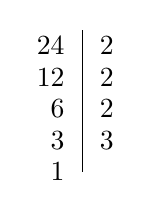
\begin{tikzpicture}[scale=1]
        % Línea vertical
        \draw (0,0.2) -- (0,-1.6);
        
        % Columna izquierda (Dividendos)
        \node[anchor=east] at (-0.1,0) {24};
        \node[anchor=east] at (-0.1,-0.4) {12};
        \node[anchor=east] at (-0.1,-0.8) {6};
        \node[anchor=east] at (-0.1,-1.2) {3};
        \node[anchor=east] at (-0.1,-1.6) {1};
        
        % Columna derecha (Divisores)
        \node[anchor=west] at (0.1,0) {2};
        \node[anchor=west] at (0.1,-0.4) {2};
        \node[anchor=west] at (0.1,-0.8) {2};
        \node[anchor=west] at (0.1,-1.2) {3};
    \end{tikzpicture}
\end{figure}

    \item \textbf{Divisor Común:} Un entero $a$ es divisor común de $b$ y de $c$ si $a$ divide a ambos; es decir, si se cumple $a \mid b$ y $a \mid c$. Por ejemplo, $2 \mid 4$ y $2 \mid 10$, así que $2$ es un divisor común de $4$ y de $10$.

    \item \textbf{Máximo Común Divisor (MCD):} El máximo común divisor de dos números enteros $a$ y $b$ se denota por $\operatorname{MCD}(a,b)$ y es el mayor divisor común a ambos números. En términos de conjuntos, corresponde al mayor valor de la intersección entre el conjunto de divisores de $a$ y el conjunto de divisores de $b$.

    \textbf{Ejemplo:} Sean $a=12$ y $b=48$. Hallamos el conjunto de divisores de cada número:
    \[ D(12)=\{1,2,3,4,6,12\} \]
    \[ D(48)=\{1,2,3,4,6,8,12,16,24,48\} \]
    Hacemos la intersección entre los conjuntos:
    \[ D(12)\cap D(48)=\{1,2,3,4,6,\fbox{12}\} \]
    El máximo valor de este conjunto corresponde al $\operatorname{MCD}(12,48)=12$. Es claro que $12 \mid 12$ y que $12 \mid 48$. En general, esto siempre se cumple: $\operatorname{MCD}(a,b) \mid a$ y $\operatorname{MCD}(a,b) \mid b$.

    \textbf{Ejemplo:} Algunas veces, cuando hemos realizado la factorización prima de los números, escogemos los factores primos \textit{comunes} con su \textit{menor exponente}. El producto de ellos corresponderá con el máximo común divisor.
    Así, para $90=2\cdot 3^2\cdot 5$ y $120=2^3\cdot 3\cdot 5$, tomamos los factores comunes con el menor exponente ($2^1$, $3^1$ y $5^1$). Por lo tanto:
    \[ \operatorname{MCD}(90,120)=2\cdot 3\cdot 5 =30 \]

    \item \textbf{Primos relativos:} Dos números $a$ y $b$ son primos relativos (o coprimos) si su máximo común divisor es $1$; es decir, $\operatorname{MCD}(a,b)=1$. Por ejemplo, $\operatorname{MCD}(80,21)= 1$, por lo tanto, $80$ y $21$ son primos relativos.\footnote{Observemos que ninguno de los dos es un número primo por sí mismo ($80$ es par y $21$ es divisible por $3$). El hecho de ser primos relativos significa que el único divisor común a ambos es el número $1$.}

    \item \textbf{Teorema (Identidad de Bézout):} Si el máximo común divisor de dos enteros $b$ y $c$ es $g=\operatorname{MCD}(b,c)$, entonces existen enteros $x_0$, $y_0$ tales que $g=bx_0+cy_0$.
    Por ejemplo, para los números $140$ y $60$, cuyo $\operatorname{MCD}$ es $20$, existen enteros $x_0$, $y_0$ que cumplen $20=140x_0+60y_0$.\footnote{¿Puedes encontrarlos? Una solución posible es $x_0=1$ y $y_0=-2$, ya que $140(1)+60(-2) = 140-120=20$.}

    Dados dos enteros $b$ y $c$, ¿cómo pueden encontrarse los valores $x_0$ y $y_0$ del teorema anterior? Si $b$ y $c$ son pequeños, $g$, $x_0$ y $y_0$ se pueden hallar por simple inspección.
    Por ejemplo, si $g=\operatorname{MCD}(10,6)=2$, buscamos satisfacer la ecuación $2=10x_0+6y_0$. Se puede observar que $x_0=2$ y $y_0=-3$ funcionan, por tanto:
    \[ 2=10(2)+6(-3) \]
    A continuación, presentamos un algoritmo que proporciona un método general para encontrar el valor de $g$ y también los coeficientes $x_0, y_0$.

    \textbf{Algoritmo de Euclides:} Dados dos enteros $b$ y $c>0$, se realiza una aplicación repetida del algoritmo de la división para obtener una serie de ecuaciones:
\begin{align}
b &= c q_1 + r_1, & 0 < r_1 < c \nonumber\\
c &= r_1 q_2 + r_2, & 0 < r_2 < r_1 \nonumber\\
r_1 &= r_2 q_3 + r_3, & 0 < r_3 < r_2 \nonumber\\
&\vdots & \nonumber \\
r_{j-2} &= r_{j-1} q_j + r_j, & 0 < r_j < r_{j-1} \nonumber\\
r_{j-1} &= r_j q_{j+1} + 0
\end{align}
El $\operatorname{MCD}(b,c)$ es $r_j$, que corresponde al \textbf{último residuo diferente de cero} en el proceso de las divisiones sucesivas. Los valores $x_0$ y $y_0$ pueden obtenerse eliminando los residuos $r_1, r_2, \dots, r_{j-1}$ mediante sustitución hacia atrás en el conjunto de ecuaciones.

\textbf{Ejemplo:} Hallar el máximo común divisor de $b=963$ y $c=657$, y encontrar los valores $x_0, y_0$ tales que $g=963x_0+657y_0$.

\textbf{Solución:} En primer lugar, aplicamos el algoritmo de Euclides mediante divisiones sucesivas:
\begin{align}
963 &= 657\cdot 1+306 \label{eq:algoritmo1}\\
657 &= 306\cdot 2+45 \label{eq:algoritmo2}\\
306 &= 45\cdot 6+36 \label{eq:algoritmo3}\\
45 &= 36\cdot 1+9 \label{eq:algoritmo4}\\
36 &= 9\cdot 4 + 0 \nonumber
\end{align}
De aquí se concluye que el máximo común divisor corresponde con el último residuo distinto de cero (ecuación \ref{eq:algoritmo4}); esto es, $\operatorname{MCD}(963,657)=9$.

Ahora, expresamos $9$ como una combinación lineal de los dos números originales. Para ello, despejamos los residuos empezando desde la ecuación (\ref{eq:algoritmo4}) y sustituyendo hacia arriba:

1. De la ecuación (\ref{eq:algoritmo4}) despejamos el 9:
\begin{equation}\label{eq:paso1}
    9 = 45 - 36 \cdot 1
\end{equation}

2. De la ecuación (\ref{eq:algoritmo3}) sabemos que $36 = 306 - 45\cdot 6$. Reemplazamos esto en (\ref{eq:paso1}):
\begin{align*}
    9 &= 45 - (306 - 45\cdot 6) \\
    9 &= 45 - 306 + 45\cdot 6 \\
    9 &= 45\cdot 7 - 306
\end{align*}

3. De la ecuación (\ref{eq:algoritmo2}) despejamos $45 = 657 - 306\cdot 2$ y reemplazamos:
\begin{align*}
    9 &= (657 - 306\cdot 2)\cdot 7 - 306 \\
    9 &= 657\cdot 7 - 306\cdot 14 - 306 \\
    9 &= 657\cdot 7 - 306\cdot 15
\end{align*}

4. Finalmente, de la ecuación (\ref{eq:algoritmo1}) despejamos $306 = 963 - 657\cdot 1$ y reemplazamos:
\begin{align*}
    9 &= 657\cdot 7 - (963 - 657)\cdot 15 \\
    9 &= 657\cdot 7 - 963\cdot 15 + 657\cdot 15 \\
    9 &= 657\cdot 22 - 963\cdot 15
\end{align*}

Así que el máximo común divisor, 9, se puede escribir como:
\[ \fbox{9 = 657(22) + 963(-15)} \]
Por tanto, $x_0 = -15$ y $y_0 = 22$.

\vspace{0.5cm}

\textbf{Mínimo Común Múltiplo:} Dado un número $a$, el conjunto de todos sus múltiplos se denota por $M(a)=\{a, 2a, 3a, \dots\}$\footnote{Es un conjunto infinito, a diferencia del conjunto de divisores que es finito.}. De la intersección entre los conjuntos de múltiplos de dos números, $M(a)\cap M(b)$, se selecciona el menor valor. Este se denominará el Mínimo Común Múltiplo, denotado como $\operatorname{MCM}(a,b)$.

\textbf{Ejemplo:} Calcular el mínimo común múltiplo de $10$ y $14$. Hallamos los conjuntos:
\begin{align*}
M(10) &= \{10,20,30,40,50,60,\fbox{70},80,90,100,110,120,130,\fbox{140},\dots\} \\
M(14) &= \{14,28,42,56,\fbox{70},84,98,112,126,\fbox{140},\dots \}
\end{align*}
La intersección es:
\begin{equation} \label{eq:interseccion}
M(10)\cap M(14) = \{70,140,\dots\}
\end{equation}
En la ecuación (\ref{eq:interseccion}) se puede ver que el conjunto de múltiplos comunes es infinito y tiene un valor mínimo que es $\operatorname{MCM}(10,14)=70$.

%==========================================================
\textbf{Teorema:} Dados dos enteros $a$ y $b$, se cumple que:
\[ \operatorname{MCM}(a,b) \cdot \operatorname{MCD}(a,b) = |ab| \]
Así, por ejemplo, sabemos que $\operatorname{MCM}(10,14)=70$ y su $\operatorname{MCD}(10,14)=2$. Entonces se verifica que:
\[ |10\cdot 14| = 140 = 70\cdot 2 \]

\section*{Ejercicios}
\begin{enumerate}
    \item Aplicando el algoritmo de Euclides, encontrar el máximo común divisor de:
    \begin{enumerate}
        \item 7469 y 2464
        \item 2689 y 4001
    \end{enumerate}
    
    \item Hallar el máximo común divisor de $1819$ y $3587$ y, a continuación, encontrar los enteros $x_0$, $y_0$ que satisfagan la ecuación:
    \[ 1819x_0 + 3587y_0 = g \]
    
    \item Encontrar valores enteros $x$, $y$ que satisfagan $93x - 81y = 3$.
\end{enumerate}

\section*{Método abreviado para hallar MCM y MCD}
En la Tabla \ref{tab:mcmmcd} se muestra el resumen del procedimiento para dos o más números naturales. 

Empezamos por el menor número primo, el $2$, y realizamos las divisiones que sean posibles. Si un número no es divisible por el primo correspondiente, se baja la cifra o se marca (en este caso con una $x$) indicando que no se operó. Luego tomamos el siguiente primo y así sucesivamente.

\begin{itemize}
    \item \textbf{Para el MCM:} Será el producto de \textbf{todos} los factores primos de la columna derecha. En este caso:
    \[ \operatorname{MCM}(160,210,100) = 2^5 \cdot 3 \cdot 5^2 \cdot 7 = 16800 \]
    \item \textbf{Para el MCD:} Se toman solo los factores primos que lograron dividir a \textbf{todos} los números de la fila simultáneamente (señalados en \textcolor{red}{rojo}). Así resulta que:
    \[ \operatorname{MCD}(160,210,100) = 2 \cdot 5 = 10 \]
\end{itemize}

\begin{table}[ht]
    \centering
    \caption{Tabla para descomposición simultánea}
    \label{tab:mcmmcd}
    \renewcommand{\arraystretch}{1.2} % Da un poco más de aire a las filas
    \begin{tabular}{|c|c|c|c|}
        \hline
        \textbf{160} & \textbf{210} & \textbf{100} & \textbf{Primos} \\ \hline
        80 & 105 & 50 & \textcolor{red}{\textbf{2}} \\ \hline
        40 & 105 & 25 & 2 \\ \hline
        20 & 105 & 25 & 2 \\ \hline
        10 & 105 & 25 & 2 \\ \hline
        5 & 105 & 25 & 2 \\ \hline
        5 & 35 & 25 & 3 \\ \hline
        1 & 7 & 5 & \textcolor{red}{\textbf{5}} \\ \hline
        1 & 7 & 1 & 5 \\ \hline
        1 & 1 & 1 & 7 \\ \hline
    \end{tabular}
\end{table}
\end{enumerate}
%=========================================================